%================================================
% PACKAGES AND THEMES
%================================================
\documentclass[t,aspectratio=169,xcolor=dvipsnames]{beamer}

\usetheme{SimplePlusAIC}

\usepackage{graphicx}
\usepackage{booktabs}
\usepackage{svg}
\usepackage{tcolorbox}
\usepackage{tikz}
\usepackage{makecell}

\newcommand*{\defeq}{\stackrel{\text{def}}{=}}
\usepackage{setspace}
\usepackage[T1]{fontenc}
\usepackage{helvet}
\usepackage{textgreek}
\usepackage{amsmath}
\usepackage{bm}
\usepackage{ragged2e}
\usepackage{xfrac}
\usepackage[loose]{units}
\usepackage{braket}
\usepackage{physics}
\usepackage{gensymb}
\usepackage{verbatim}
\usepackage{fancyvrb}

\usepackage[svgnames,table]{xcolor}
\arrayrulecolor{black}
\setlength{\arrayrulewidth}{0.20mm}
\renewcommand{\arraystretch}{1.35}

\newcommand{\tem}[1]{\textbf{\textcolor{red}{#1}}}

%================================================
% TITLE PAGE
%================================================
\title[Virtual Memory]{Virtual Memory}
\subtitle{Week 5: Penjelasan Step-by-Step}
\author[lectura.id/course/os]{lectura.id/course/os}
\institute[ITERA]{Program Studi Teknik Informatika \\ Institut Teknologi Sumatera}
\date{\textcolor{nyublue}{2026}}

%================================================
% BEGIN DOCUMENT
%================================================
\begin{document}

\begin{frame}
    \titlepage
\end{frame}

\begin{frame}
    \frametitle{OUTLINE}
    \framesubtitle{Peta materi pertemuan ini}
    \small
    \begin{spacing}{1.15}
        \tableofcontents
    \end{spacing}
\end{frame}

\begin{frame}
    \frametitle{Capaian Pembelajaran}
    \framesubtitle{Tujuan setelah pertemuan selesai}
    \small
    \begin{enumerate}
        \item Menjelaskan kenapa virtual memory dibutuhkan.
        \item Memahami address space dengan contoh sederhana.
        \item Menelusuri translasi alamat langkah demi langkah.
        \item Memahami segmentasi dan masalah fragmentasi.
        \item Memahami dasar allocator: split, coalesce, fit policy.
    \end{enumerate}
    \begin{exampleblock}{Fokus Kelas Ini}
        Kita belajar pelan-pelan, \tem{dari konsep paling dasar} sampai mekanisme yang dipakai OS modern.
    \end{exampleblock}
\end{frame}

\begin{frame}
    \frametitle{Cara Belajar Hari Ini}
    \framesubtitle{Supaya materi tidak terasa berat}
    \small
    \begin{enumerate}
        \item Lihat dulu masalahnya (kenapa VM perlu).
        \item Pahami istilah satu per satu.
        \item Ikuti contoh hitung sederhana.
        \item Cek pemahaman lewat pertanyaan pendek.
        \item Ulangi dengan analogi kehidupan sehari-hari.
    \end{enumerate}
    \begin{alertblock}{Aturan Main Kelas}
        Jika ada satu langkah belum paham, jangan lanjut dulu ke langkah berikutnya.
    \end{alertblock}
\end{frame}

\section{Mengapa Virtual Memory?}

\begin{frame}
    \frametitle{Masalah Dasar Tanpa Virtual Memory}
    \framesubtitle{Apa yang rusak jika semua proses menyentuh RAM langsung?}
    \small
    \begin{itemize}
        \item Proses A bisa menimpa data proses B.
        \item Programmer harus tahu alamat fisik asli (sulit sekali).
        \item Sulit memindah proses saat sistem ramai.
    \end{itemize}
    \vspace{0.2cm}
    \begin{alertblock}{Inti Masalah}
        Banyak proses, satu RAM fisik. Bagaimana caranya tetap aman, adil, dan mudah diprogram?
    \end{alertblock}
\end{frame}

\begin{frame}
    \frametitle{Analogi Sederhana: Apartemen}
    \framesubtitle{Cara mudah membayangkan virtual memory}
    \small
    Bayangkan RAM seperti apartemen besar:
    \begin{enumerate}
        \item Banyak penghuni (proses) tinggal di satu gedung (RAM fisik).
        \item Tiap penghuni merasa punya unit sendiri (address space virtual).
        \item Satpam dan pengelola gedung (hardware + OS) mencegah pelanggaran.
    \end{enumerate}
    \begin{exampleblock}{Makna Analogi}
        \tem{Virtual memory = ilusi yang terkontrol.} Ilusi ini membuat hidup programmer jauh lebih mudah.
    \end{exampleblock}
\end{frame}

\begin{frame}
    \frametitle{Dari Sistem Lama ke Multiprogramming}
    \framesubtitle{Perubahan kebutuhan dari 1 proses ke banyak proses}
    \small
    \begin{columns}[T]
        \column{0.48\textwidth}
        \centering
        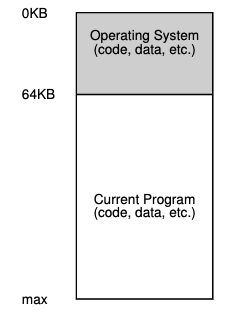
\includegraphics[width=\textwidth,height=0.45\textheight,keepaspectratio]{../2_Book_Translate/figures/6_1.png}

        \textbf{Sistem awal:} OS + satu program, sederhana tapi tidak skalabel.

        \column{0.48\textwidth}
        \centering
        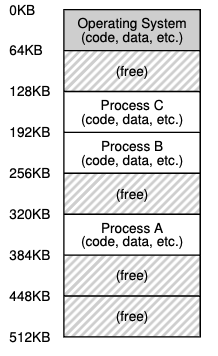
\includegraphics[width=\textwidth,height=0.45\textheight,keepaspectratio]{../2_Book_Translate/figures/6_2.png}

        \textbf{Multiprogramming:} banyak proses aktif, butuh isolasi dan proteksi.
    \end{columns}
\end{frame}

\begin{frame}
    \frametitle{Address Space Proses}
    \framesubtitle{Struktur memori yang dilihat program}
    \small
    \begin{columns}[T]
        \column{0.42\textwidth}
        \centering
        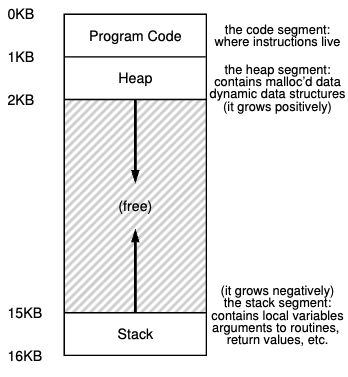
\includegraphics[width=\textwidth,height=0.58\textheight,keepaspectratio]{../2_Book_Translate/figures/6_3.png}
        \column{0.55\textwidth}
        \begin{itemize}
            \item \textbf{Code}: instruksi program.
            \item \textbf{Data}: variabel global/statis.
            \item \textbf{Heap}: alokasi dinamis, cenderung tumbuh ke atas.
            \item \textbf{Stack}: frame fungsi, cenderung tumbuh ke bawah.
        \end{itemize}
        \vspace{0.2cm}
        Program hanya melihat peta virtual ini. OS yang menghubungkan ke RAM fisik.
    \end{columns}
\end{frame}

\begin{frame}
    \frametitle{Checkpoint 1}
    \framesubtitle{Cek pemahaman sebelum lanjut}
    \small
    \begin{enumerate}
        \item Kenapa proses A tidak boleh menulis ke memori proses B?
        \item Kenapa programmer sebaiknya tidak mengatur alamat fisik langsung?
        \item Apa bedanya RAM fisik dengan address space virtual?
    \end{enumerate}
    \begin{block}{Kunci Jawaban Singkat}
        VM ada untuk \tem{isolasi}, \tem{kemudahan}, dan \tem{fleksibilitas}.
    \end{block}
\end{frame}

\section{API Memori (C) Secara Praktis}

\begin{frame}
    \frametitle{Stack vs Heap (Pelan-Pelan)}
    \framesubtitle{Ini pondasi sebelum bicara allocator}
    \small
    \begin{table}[]
        \centering
        \begin{tabular}{p{0.20\textwidth}p{0.33\textwidth}p{0.37\textwidth}}
            \toprule
            \textbf{Aspek} & \textbf{Stack} & \textbf{Heap} \\
            \midrule
            Cara alokasi & Otomatis saat fungsi dipanggil & Manual lewat \texttt{malloc()} \\
            Kapan hilang & Otomatis saat fungsi selesai & Harus dipanggil \texttt{free()} \\
            Cepat/lambat & Umumnya lebih cepat & Lebih fleksibel, tapi perlu pengelolaan \\
            Risiko bug & Stack overflow & Leak, double free, dangling pointer \\
            \bottomrule
        \end{tabular}
    \end{table}
\end{frame}

\begin{frame}
    \frametitle{Langkah Aman Pakai \texttt{malloc/free}}
    \framesubtitle{Urutan kerja yang sebaiknya selalu diikuti}
    \small
    \begin{enumerate}
        \item Tentukan ukuran data yang benar.
        \item Panggil \texttt{malloc(size)}.
        \item Cek apakah hasilnya \texttt{NULL}.
        \item Gunakan memori sesuai batas ukuran.
        \item Panggil \texttt{free(ptr)} saat selesai.
        \item Set pointer menjadi \texttt{NULL}.
    \end{enumerate}
    \begin{exampleblock}{Kenapa langkah 6 penting?}
        Supaya pointer lama tidak dipakai lagi secara tidak sengaja (mencegah dangling pointer).
    \end{exampleblock}
\end{frame}

\begin{frame}
    \frametitle{Bug 1: Memory Leak dan Double Free}
    \framesubtitle{Dua bug klasik yang sering muncul}
    \small
    \textbf{Memory Leak}
    \begin{itemize}
        \item Terjadi saat memori sudah diminta, tapi tidak pernah dikembalikan.
        \item Dampak: aplikasi makin lama makin boros RAM.
    \end{itemize}

    \textbf{Double Free}
    \begin{itemize}
        \item Terjadi saat pointer yang sama di-\texttt{free()} lebih dari sekali.
        \item Dampak: struktur allocator bisa rusak, program crash.
    \end{itemize}
\end{frame}

\begin{frame}
    \frametitle{Bug 2: Dangling Pointer dan Out-of-Bounds}
    \framesubtitle{Bug yang sering sulit dideteksi}
    \small
    \textbf{Dangling Pointer}
    \begin{itemize}
        \item Pointer masih dipakai padahal memorinya sudah dibebaskan.
    \end{itemize}

    \textbf{Out-of-Bounds}
    \begin{itemize}
        \item Menulis lewat batas buffer (misal index terlalu besar).
        \item Bisa merusak data lain di memori.
    \end{itemize}

    \begin{alertblock}{Checklist Cepat}
        Validasi ukuran, validasi index, dan disiplin pada siklus hidup pointer.
    \end{alertblock}
\end{frame}

\begin{frame}
    \frametitle{Checkpoint 2}
    \framesubtitle{Pastikan pondasi API memori sudah kuat}
    \small
    \begin{enumerate}
        \item Apa beda umur data pada stack dan heap?
        \item Kenapa \texttt{free()} wajib dipanggil?
        \item Kenapa pointer sebaiknya diset ke \texttt{NULL} setelah \texttt{free()}?
    \end{enumerate}
\end{frame}

\begin{frame}
    \frametitle{Video Pendukung (API Memori C)}
    \framesubtitle{Cocok ditonton di rumah}
    \small
    \textbf{How to manage memory with malloc, calloc, realloc, and free in C}\\
    \scriptsize \url{https://www.youtube.com/watch?v=lQP4X3odvHE}
    \normalsize
    \vspace{0.2cm}
    Fokus pada pola aman \texttt{malloc()} $\rightarrow$ pakai sesuai batas $\rightarrow$ \texttt{free()}.
\end{frame}

\section{Mekanisme Translasi Alamat}

\begin{frame}
    \frametitle{Apa Itu Translasi Alamat?}
    \framesubtitle{Inti kerja VM di level hardware}
    \small
    Saat program mengakses alamat, yang keluar dari CPU adalah \textbf{alamat virtual}, bukan alamat fisik.

    \vspace{0.2cm}
    Hardware Memory Management Unit (MMU) melakukan:
    \begin{enumerate}
        \item Cek valid/tidaknya alamat.
        \item Hitung alamat fisik yang sebenarnya.
        \item Raise exception jika akses tidak legal.
    \end{enumerate}
\end{frame}

\begin{frame}
    \frametitle{Base-and-Bounds: Konsep Dasar}
    \framesubtitle{Model translasi yang paling mudah dipahami}
    \small
    Dua register penting:
    \begin{itemize}
        \item \textbf{Base}: titik awal memori fisik proses.
        \item \textbf{Bounds}: ukuran area legal proses.
    \end{itemize}

    Rumus saat valid:
    \[\text{Physical Address} = \text{Base} + \text{Virtual Address}\]

    Jika tidak valid (melewati bounds), maka trap ke OS.
\end{frame}

\begin{frame}
    \frametitle{Translasi Langkah Demi Langkah}
    \framesubtitle{Step 1 sampai Step 4}
    \small
    \begin{columns}[T]
        \column{0.48\textwidth}
        \begin{enumerate}
            \item Proses meminta alamat virtual \texttt{V}.
            \item Hardware cek: \texttt{V < bounds}? 
            \item Jika benar: hitung \texttt{base + V}.
            \item Jika salah: kirim exception ke kernel.
        \end{enumerate}
        \vspace{0.2cm}
        \textbf{Makna:} proteksi berjalan otomatis, tidak menunggu aplikasi sadar salah.

        \column{0.50\textwidth}
        \centering
        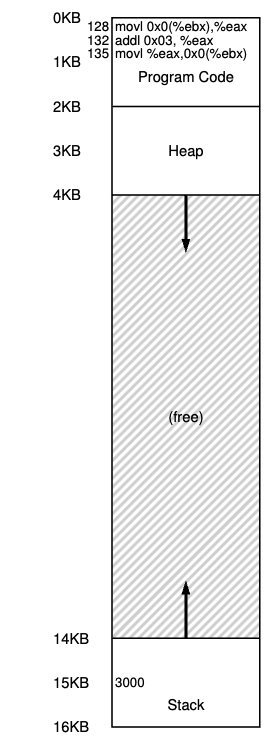
\includegraphics[width=\textwidth,height=0.66\textheight,keepaspectratio]{../2_Book_Translate/figures/6_4.png}
    \end{columns}
\end{frame}

\begin{frame}
    \frametitle{Contoh Hitung Translasi}
    \framesubtitle{Latihan angka sederhana}
    \small
    Diketahui \texttt{base = 4000}, \texttt{bounds = 1000}.
    \begin{table}[]
        \centering
        \begin{tabular}{ccc}
            \toprule
            \textbf{V} & \textbf{Valid?} & \textbf{Alamat Fisik} \\
            \midrule
            120 & Ya & 4120 \\
            980 & Ya & 4980 \\
            1200 & Tidak & Trap \\
            \bottomrule
        \end{tabular}
    \end{table}
    \begin{exampleblock}{Ingat}
        \texttt{V} boleh kecil, tapi tetap harus dicek terhadap \texttt{bounds} setiap akses.
    \end{exampleblock}
\end{frame}

\begin{frame}
    \frametitle{Apa yang Terjadi Saat Trap?}
    \framesubtitle{Alur saat proses melanggar batas}
    \small
    \begin{columns}[T]
        \column{0.46\textwidth}
        \begin{enumerate}
            \item Hardware mendeteksi akses ilegal.
            \item Hardware menghentikan sementara proses user.
            \item Kontrol pindah ke kernel (exception handler).
            \item OS memutuskan tindakan: hentikan proses, kirim sinyal error, dll.
        \end{enumerate}
        \column{0.52\textwidth}
        \centering
        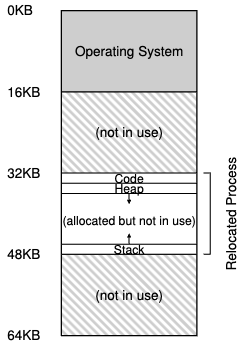
\includegraphics[width=\textwidth,height=0.68\textheight,keepaspectratio]{../2_Book_Translate/figures/6_5.png}
    \end{columns}
\end{frame}

\begin{frame}
    \frametitle{Kerja Sama Hardware dan OS}
    \framesubtitle{Mekanisme cepat + kebijakan aman}
    \scriptsize
    \begin{table}[]
        \centering
        \begin{tabular}{p{0.30\textwidth}p{0.62\textwidth}}
            \toprule
            \textbf{Komponen} & \textbf{Peran} \\
            \midrule
            Hardware & Translasi alamat, cek bounds, dan trap secara cepat. \\
            Hardware & Menyediakan mode privileged untuk instruksi sensitif. \\
            OS & Mengisi register base/bounds saat context switch. \\
            OS & Menyiapkan dan menjalankan handler exception. \\
            OS & Mengalokasikan dan membebaskan memori proses. \\
            \bottomrule
        \end{tabular}
    \end{table}
\end{frame}

\begin{frame}
    \frametitle{Checkpoint 3}
    \framesubtitle{Evaluasi cepat bagian translasi}
    \small
    \begin{enumerate}
        \item Kenapa translasi sebaiknya dilakukan hardware, bukan software murni?
        \item Kapan trap terjadi pada base-and-bounds?
        \item Saat context switch, kenapa register base/bounds harus diperbarui?
    \end{enumerate}
\end{frame}

\begin{frame}
    \frametitle{Video Pendukung (Translasi Alamat)}
    \framesubtitle{Cocok ditonton di rumah}
    \small
    \begin{enumerate}
        \item \textbf{Mechanism of Address Translation}\\
        \scriptsize \url{https://www.youtube.com/watch?v=mYxkp5vpyqc}
    \end{enumerate}
\end{frame}

\section{Segmentasi}

\begin{frame}
    \frametitle{Mengapa Segmentasi Diperlukan?}
    \framesubtitle{Kelemahan model satu blok kontigu}
    \small
    Jika satu address space diperlakukan sebagai satu blok:
    \begin{itemize}
        \item Banyak ruang kosong ikut terbawa ke RAM fisik.
        \item Pemakaian RAM jadi boros.
    \end{itemize}

    Segmentasi membagi address space menjadi bagian logis:
    \begin{itemize}
        \item Code
        \item Heap
        \item Stack
    \end{itemize}
\end{frame}

\begin{frame}
    \frametitle{Cara Membaca Alamat pada Segmentasi}
    \framesubtitle{Langkah 1 sampai 4}
    \small
    \begin{enumerate}
        \item Ambil bit atas untuk menentukan nomor segmen.
        \item Ambil sisa bit sebagai offset dalam segmen itu.
        \item Cek offset apakah masih dalam size segmen.
        \item Jika valid, hitung alamat fisik = base segmen + offset.
    \end{enumerate}

    \begin{exampleblock}{Keuntungan}
        Tiap segmen bisa dipindah atau diatur sendiri, jadi lebih fleksibel daripada satu blok besar.
    \end{exampleblock}
\end{frame}

\begin{frame}
    \frametitle{Contoh Segmentasi di Memori Fisik}
    \framesubtitle{Visual kiri-kanan: ruang virtual vs penempatan fisik}
    \small
    \begin{columns}[T]
        \column{0.49\textwidth}
        \centering
        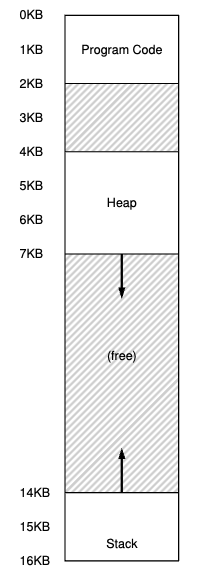
\includegraphics[width=0.98\textwidth,height=0.64\textheight,keepaspectratio]{../2_Book_Translate/figures/6_7.png}

        {\scriptsize \textbf{(Kiri)} Address space proses dengan celah ruang.}

        \column{0.49\textwidth}
        \centering
        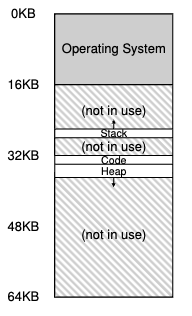
\includegraphics[width=0.98\textwidth,height=0.64\textheight,keepaspectratio]{../2_Book_Translate/figures/6_8.png}

        {\scriptsize \textbf{(Kanan)} Segmen ditempatkan terpisah di RAM fisik.}
    \end{columns}
\end{frame}

\begin{frame}
    \frametitle{Contoh Nilai Register Segmen}
    \framesubtitle{Supaya tidak abstrak}
    \small
    \begin{table}[]
        \centering
        \begin{tabular}{lcc}
            \toprule
            \textbf{Segment} & \textbf{Base} & \textbf{Size} \\
            \midrule
            Code & 32K & 2K \\
            Heap & 34K & 3K \\
            Stack & 28K & 2K \\
            \bottomrule
        \end{tabular}
    \end{table}
    \vspace{0.2cm}
    \textbf{Contoh cepat:} jika offset heap = 1K, alamat fisik heap = 34K + 1K = 35K (jika masih dalam size).
\end{frame}

\begin{frame}
    \frametitle{Fragmentasi Eksternal dan Compaction}
    \framesubtitle{Masalah utama pada segmentasi}
    \small
    \begin{columns}[T]
        \column{0.50\textwidth}
        \begin{itemize}
            \item Ruang kosong total bisa banyak.
            \item Tapi ruang itu tersebar jadi potongan kecil.
            \item Request besar bisa gagal meskipun total kosong cukup.
            \item Compaction menggabungkan ruang kosong, tapi mahal.
        \end{itemize}
        \column{0.47\textwidth}
        \centering
        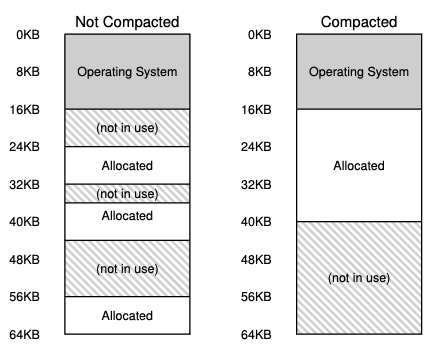
\includegraphics[width=\textwidth,height=0.55\textheight,keepaspectratio]{../2_Book_Translate/figures/6_10.png}
    \end{columns}
\end{frame}

\begin{frame}
    \frametitle{Checkpoint 4}
    \framesubtitle{Pastikan segmentasi sudah masuk}
    \small
    \begin{enumerate}
        \item Kenapa segmentasi bisa lebih hemat dibanding satu blok besar?
        \item Kenapa tetap bisa muncul fragmentasi eksternal?
        \item Kenapa compaction tidak dilakukan terus-menerus?
    \end{enumerate}
\end{frame}

\begin{frame}
    \frametitle{Video Pendukung (Segmentasi)}
    \framesubtitle{Cocok ditonton di rumah}
    \small
    \textbf{Operating Systems Lecture: Main Memory (Segmentation)}\\
    \scriptsize \url{https://www.youtube.com/watch?v=akADkYH5M8o}
    \normalsize
    \vspace{0.2cm}
    Cocok untuk menguatkan konsep \textit{base/size} per segmen.
\end{frame}

\section{Manajemen Free-Space}

\begin{frame}
    \frametitle{Masalah di Allocator}
    \framesubtitle{Permintaan ukuran memori berubah-ubah}
    \small
    Tantangan allocator:
    \begin{itemize}
        \item Ukuran request tidak tetap (kecil, sedang, besar).
        \item Blok kosong bisa terpecah-pecah.
        \item Harus cepat, tapi juga hemat ruang.
    \end{itemize}
    \begin{alertblock}{Trade-off Inti}
        Waktu alokasi cepat sering berlawanan dengan kualitas tata ruang jangka panjang.
    \end{alertblock}
\end{frame}

\begin{frame}
    \frametitle{Header Blok pada Heap}
    \framesubtitle{Metadata kecil yang sangat penting}
    \small
    \begin{center}
        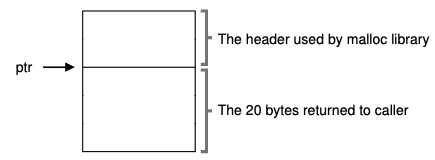
\includegraphics[width=0.46\textwidth,height=0.32\textheight,keepaspectratio]{../2_Book_Translate/figures/6_11a.png}
        \hspace{0.02\textwidth}
        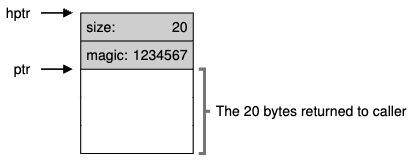
\includegraphics[width=0.46\textwidth,height=0.32\textheight,keepaspectratio]{../2_Book_Translate/figures/6_11b.png}
    \end{center}
    \vspace{0.2cm}
    Header menyimpan info seperti ukuran blok dan status (dipakai/kosong), agar \texttt{free()} dapat bekerja benar.
\end{frame}

\begin{frame}
    \frametitle{Perubahan Heap Saat Alokasi Awal}
    \framesubtitle{Visual step-by-step sebelum dan sesudah alokasi}
    \small
    \begin{center}
        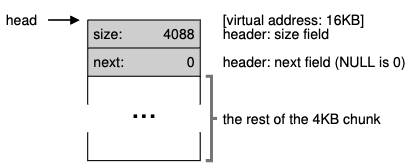
\includegraphics[width=0.46\textwidth,height=0.32\textheight,keepaspectratio]{../2_Book_Translate/figures/6_12a.png}
        \hspace{0.02\textwidth}
        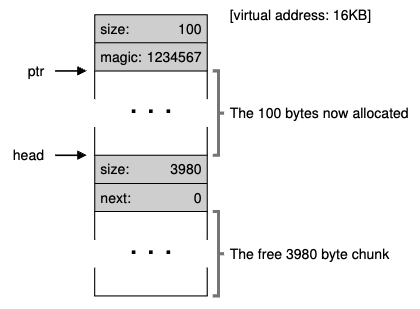
\includegraphics[width=0.46\textwidth,height=0.32\textheight,keepaspectratio]{../2_Book_Translate/figures/6_12b.png}
    \end{center}
    \vspace{0.2cm}
    \begin{enumerate}
        \item Allocator menemukan blok kosong.
        \item Jika terlalu besar, blok di-\textit{split}.
        \item Bagian yang dipakai diberikan ke user.
        \item Sisanya tetap masuk free list.
    \end{enumerate}
\end{frame}

\begin{frame}
    \frametitle{Strategi Fit: First, Best, Worst}
    \framesubtitle{Kebijakan memilih blok kosong}
    \small
    \begin{table}[]
        \centering
        \begin{tabular}{p{0.20\textwidth}p{0.33\textwidth}p{0.37\textwidth}}
            \toprule
            \textbf{Strategi} & \textbf{Kelebihan} & \textbf{Kekurangan} \\
            \midrule
            First Fit & Cepat, sederhana & Cenderung cepat membuat pecahan blok \\
            Best Fit & Sisa blok lokal kecil & Proses pencarian lebih lama \\
            Worst Fit & Menyisakan blok besar & Tidak selalu stabil di praktik \\
            \bottomrule
        \end{tabular}
    \end{table}
\end{frame}

\begin{frame}
    \frametitle{Coalescing dan Buddy System}
    \framesubtitle{Dua cara menjaga kualitas free-space}
    \small
    \begin{columns}[T]
        \column{0.48\textwidth}
        \centering
        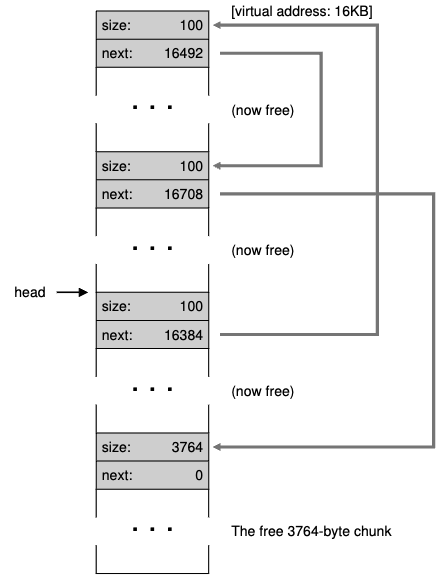
\includegraphics[width=\textwidth,height=0.46\textheight,keepaspectratio]{../2_Book_Translate/figures/6_13.png}

        \textbf{Coalescing:} gabung blok kosong bertetangga agar request besar tetap mungkin.

        \column{0.48\textwidth}
        \centering
        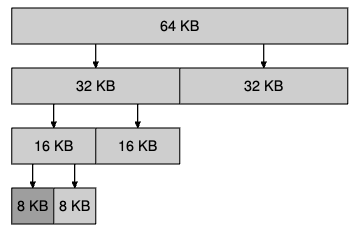
\includegraphics[width=\textwidth,height=0.46\textheight,keepaspectratio]{../2_Book_Translate/figures/6_14.png}

        \textbf{Buddy:} pembagian terstruktur (umumnya pangkat dua), merge lebih cepat tapi bisa internal fragmentation.
    \end{columns}
\end{frame}

\begin{frame}
    \frametitle{Checkpoint 5}
    \framesubtitle{Penutup bagian allocator}
    \small
    \begin{enumerate}
        \item Kenapa free list tanpa coalescing bisa jadi buruk?
        \item Kapan best fit terlihat menarik? Kapan justru merugikan?
        \item Apa trade-off utama buddy system?
    \end{enumerate}
\end{frame}

\begin{frame}
    \frametitle{Video Pendukung (Free-Space Management)}
    \framesubtitle{Cocok ditonton di rumah}
    \small
    \begin{enumerate}
        \item \textbf{Memory Allocation and Free Space Management Algorithms}\\
        \scriptsize \url{https://youtu.be/bq3_uT5Z424}
        \normalsize
        \item \textbf{Playlist OS (cadangan belajar mandiri)}\\
        \scriptsize \url{https://www.youtube.com/playlist?list=PLDW872573QAb4bj0URobvQTD41IV6gRkx}
    \end{enumerate}
\end{frame}

\section{Ringkasan dan Latihan}

\begin{frame}
    \frametitle{Ringkasan Super Singkat (6 Kalimat Kunci)}
    \framesubtitle{Jika lupa materi, ingat 6 poin ini}
    \small
    \begin{enumerate}
        \item VM memberi ilusi memori privat per proses.
        \item Translasi alamat dilakukan hardware sangat sering.
        \item Base-and-bounds memberi proteksi cepat dan sederhana.
        \item Segmentasi menambah fleksibilitas tata letak memori.
        \item Free-space management menjaga alokasi ukuran variabel tetap sehat.
        \item Semua desain memori adalah trade-off performa vs efisiensi ruang.
    \end{enumerate}
\end{frame}

\begin{frame}
    \frametitle{Latihan Mandiri Step-by-Step}
    \framesubtitle{Kerjakan pelan, diskusikan berpasangan}
    \small
    \begin{enumerate}
        \item Diketahui \texttt{base=5000}, \texttt{bounds=700}. Apakah \texttt{V=650} valid? Jika valid, berapa alamat fisiknya?
        \item Sebutkan 2 contoh bug heap dan cara pencegahannya.
        \item Jelaskan kenapa segmentasi dapat mengurangi pemborosan, tetapi tetap berpotensi fragmentasi eksternal.
        \item Jika blok kosong: 12KB, 7KB, 4KB dan request 3KB, strategi fit mana yang Anda pilih? Jelaskan alasan.
    \end{enumerate}
\end{frame}

\begin{frame}
    \frametitle{Terima Kasih}
    \begin{center}
        \Huge \textbf{Ada Pertanyaan?}

        \vspace{0.8cm}
        \normalsize
        Ulangi kembali 5 checkpoint tadi. Jika 1 checkpoint masih belum paham, mulai dari bagian itu.
    \end{center}
\end{frame}

\end{document}
